\chapter{Trave: momento flettente SLU}
\section{Progetto della sezione maggiormente sollecitata}
In riferimento ai valori mostrati in precedenza nella tabella \ref{tab:trave_ULS_momento} a pagina \pageref{tab:trave_ULS_momento}, si progetta ora la sezione in calcestruzzo armato considerando quella maggiormente sollecitata.
Nel caso in esame è quella in appoggio 5 avente un momento pari a $\SI{-247.45}{\kilo\newton\metre}$.
Essendo soggetta a momento flettente negativo, sarà considerata invertita rispetto la dispozione reale e considerata quindi a momento flettente positivo, con le amrature invertite. 
A tale scopo verrà utilizzata la nomenclatura \emph{inv.} nelle tabelle a seguire per indicare tutte quelle sezioni che sono state inveritite.

\begin{figure}[ht]
  \centering
  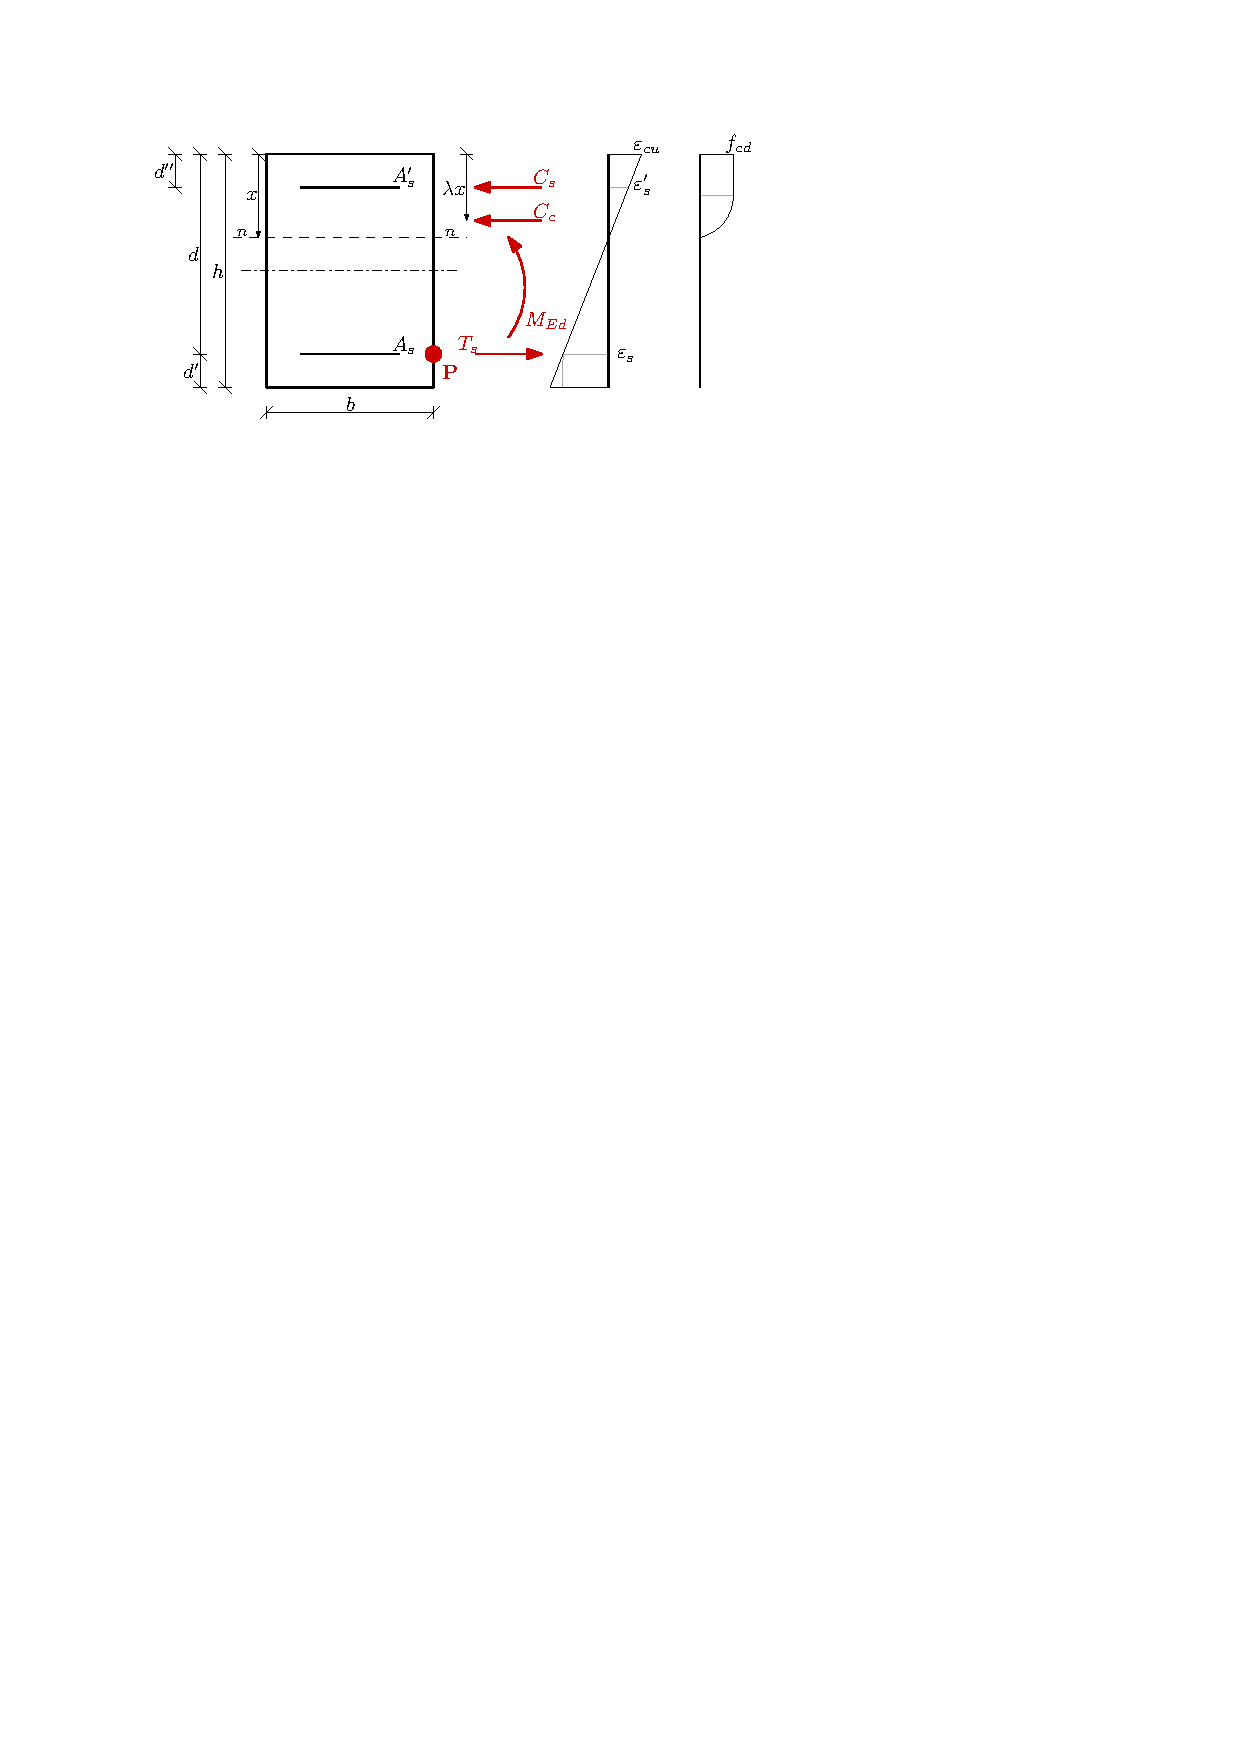
\includegraphics[height=0.25\textheight]{IMG/IPE_slu_progetto.pdf}
  \caption{Convenzione e nomenclatura utilizzata per il progetto agli SLU}
  \label{fig:slu_progetto}
\end{figure}

Utilizzando la convenzione di segni riportata in figura \ref{fig:slu_progetto} e il polo $\mathbf{P}$ riportato, è possibile scrivere il sistema per determinare i valori dell'altezza utile $d$ e della quantita di armature inferiori $A_s$ che soddisfano il momento flettente applicato. 
\begin{equation}
  \begin{cases}
    C_c + C_s - T_s = 0 \\
    C_c \left(d - \lambda\,x\right) + C_s \left(d - d^{\prime\prime}\right) = M_{Ed}
  \end{cases}
\end{equation}
Sistema che è possibile risolvere esplicitando i valori delle risultanti e facendo delle ipotesi per ridurrre il numero di variabili. 
Si fissa il rapporto di armatura $\beta = 0.2$, ovvero pari al minimo possibile, in quanto il momente flettente a segno opposto nella sezione in esame è nullo.
Inoltre il progetto è vincolato, pertanto la base è imposta a \SI{300}{\milli\metre}.
Come copriferri $d^\prime,d^{\prime\prime}$ si scelgono entrambi uguali e pari a \SI{40}{\milli\metre}.
Infine si fissa il pieno utilizzo delle capacità meccaniche dei materiali: per cui l'acciaio superiore risulta snervato, e di conseguenza $\sigma_s^\prime = f_{yd}$, e il calcestruzzo a collasso, e di conseguenza $\sigma_c = f_{cd}$.
I coefficienti $\lambda$ e $\psi$ sono quelli del campo 3 e quindi pari a $\frac{17}{21}$ e $\frac{99}{238}$.

Il sistema espanso risulta:
\begin{equation}
  \begin{cases}
    b \, \psi \, \xi \, d \, f_{cd} + \beta \, A_s \, f_{yd} - A_s \, f_{yd} = 0 \\
    b \, \psi \, \xi \, d \, f_{cd} \left(d - \lambda\,x\right) + \beta \, A_s \, f_{yd} \left(d - d^{\prime\prime}\right) = M_{Ed}
  \end{cases}
\end{equation}
e risolvendolo si ottengono i seguenti valori:
\begin{equation}
  \hookrightarrow \quad
  \begin{cases}
    A_s &= \SI{1416.82}{\milli\metre\squared} \\
    A_s^\prime &= \SI{283.36}{\milli\metre\squared} \\
    d &= \SI{497.23}{\milli\metre}
  \end{cases}
\end{equation}

Si vuole cercare di avere un'altezza totale $h = \SI{500}{\milli\metre}$, per cui si sceglie un'altezza utile $d = \SI{460}{\milli\metre}$ inferiore a quella ottenuta dal sistema. 
I valori di armature $A_s$ sono soddisfatti con ad esempio 8Ø16, 6Ø18 o 5Ø20, aventi rispettivamente \SI{1608}, \SI{1527}, \SI{1570}{\milli\metre\squared} di area.
Avendo problemi riguardo la base minima su cui si dispongono le barre, il diametro da 16 non può essere utilizzato. 
Vengono perciò adottati i 6Ø18 che rispettano i requisiti, come di seguito dimostrato:
\begin{equation}  
  \begin{split}
    b_{min} &= 2 \cdot \text{copriferro} + 2 \cdot \varnothing_\textup{staffe} + n_\textup{barre} \cdot \varnothing_\textup{barre} + \left( n_\textup{barre} - 1 \right) \cdot \text{dist}_\textup{barre}  \\
    &= 2 \cdot 20 + 2 \cdot 10 + 6 \cdot 18 + \left( 6 - 1 \right) \cdot 25 \quad \si{\milli\metre}\\
    &= \SI{293}{\milli\metre} < b = \SI{300}{\milli\metre} \quad \checkmark ,
  \end{split}
\end{equation}
mentre per le armature superiori si scelgono 2Ø18 con unica funzione di reggistaffa.

\subsection{Verifica della sezione maggiormente sollecitata}
%--- LOG --- 
%Ipotesi di campo 3B, calcolo della retta limite 2-3
%xi_23 = 0.25926
%Esiste campo 2a, 2b, 3b perchè d2 = 40.00 < d2_xi23 = 55.77 mm
%xi_3 = 0.25166
%Ipotesi di campo 3 errata! xi_3 = 0.25166 < xi_23 = 0.25926 ma devo comunque verificare tramite es1 perché ho usato hp di es plasticizzato del 3B
%Essendo d2 = 40.00000 < d2_xi23 = 55.76720, non può esserci il campo 3A
%Calcolo xi con ipotesi di campo 2B: armature superiori snervate
%xi_2b = 0.25349
%!!!!!!!!!!!!!!verifica del ec da fare
%Ipotesi armature superiori snervate ok! es1 = 0.22308% > di ese1 = 0.18634%

%campo': '2B',
% 'ec': 0.0033956711163810735,
% 'es': 0.01,
% 'es1': 0.002230830149739241,
% 'xi': 0.2534901825283417,
% 'psi': 0.8036716031035525,
% 'lamb': 0.4138260346516767,
% 'Nrd': 0.0,
% 'Mrd': 247633547.16419485

  \begin{table}[htb]
    \centering
    \scriptsize
    \caption{ULS}
    \begin{tabular}{
        l
        c
        c
        S[table-format=3.3]
        l
        S[table-format=2.2]
        S[table-format=2.2]
        S[table-format=2.2]
        S[table-format=1.4]
        S[table-format=1.4]
        S[table-format=1.4]
        S[table-format=3.3]
        r
        S[table-format=2.1]}
    \toprule
    \multirow{2}{*}{Sez.}   & \multirow{2}{*}{$A_s$}    & \multirow{2}{*}{$A_s^\prime$} & {$M_{Ed}$}                    & \multirow{2}{*}{Campo}    & {$\varepsilon_c$}         & {$\varepsilon_s$}         & {$\varepsilon_s^\prime$}  & \multicolumn{1}{c}{\multirow{2}{*}{$\xi$}}    & \multicolumn{1}{c}{\multirow{2}{*}{$\psi$}}   & \multicolumn{1}{c}{\multirow{2}{*}{$\lambda$}}    & {$M_{Rd}$}                    & \multicolumn{2}{l}{$M_{Ed}<M_{Rd}$} \\
                            &                           &                               & {\si{[\kilo\newton\metre]}}   &                           &{\si{[\textperthousand]}}  &{\si{[\textperthousand]}}  &  {\si{[\textperthousand]}} &                        &                           &                               & {\si{[\kilo\newton\metre]}}   & & {\si{[\percent]}}\\
    \midrule
    A1 inv & 2Ø18 & 2Ø18 & 0.000   & 2A-1 & 1.51 & 10.00 & 0.51 & 0.1311 & 0.5648 & 0.3613 & 86.276  & \checkmark & 0.0 \\
    C1     & 3Ø18 & 2Ø18 & 90.595  & 2A-1 & 1.91 & 10.00 & 0.88 & 0.1607 & 0.6519 & 0.3724 & 128.015 & \checkmark & 70.8 \\
    A2 inv & 6Ø18 & 2Ø18 & 190.969 & 2B   & 3.40 & 10.00 & 2.23 & 0.2535 & 0.8037 & 0.4138 & 247.634 & \checkmark & 77.1 \\
    C2     & 4Ø18 & 2Ø18 & 149.180 & 2A-2 & 2.33 & 10.00 & 1.26 & 0.1890 & 0.7139 & 0.3856 & 168.988 & \checkmark & 88.3 \\
    A3 inv & 6Ø18 & 2Ø18 & 209.462 & 2B   & 3.40 & 10.00 & 2.23 & 0.2535 & 0.8037 & 0.4138 & 247.634 & \checkmark & 84.6 \\
    C3     & 3Ø18 & 2Ø18 & 120.204 & 2A-1 & 1.91 & 10.00 & 0.88 & 0.1607 & 0.6519 & 0.3724 & 128.015 & \checkmark & 93.9 \\
    A4 inv & 6Ø18 & 2Ø18 & 196.601 & 2B   & 3.40 & 10.00 & 2.23 & 0.2535 & 0.8037 & 0.4138 & 247.634 & \checkmark & 79.4 \\
    C4     & 4Ø18 & 2Ø18 & 139.165 & 2A-2 & 2.33 & 10.00 & 1.26 & 0.1890 & 0.7139 & 0.3856 & 168.988 & \checkmark & 82.4 \\
    A5 inv & 6Ø18 & 2Ø18 & 247.450 & 2B   & 3.40 & 10.00 & 2.23 & 0.2535 & 0.8037 & 0.4138 & 247.634 & \checkmark & 99.9 \\
    C5     & 4Ø18 & 2Ø18 & 162.530 & 2A-2 & 2.33 & 10.00 & 1.26 & 0.1890 & 0.7139 & 0.3856 & 168.988 & \checkmark & 96.2 \\
    A6 inv & 6Ø18 & 2Ø18 & 204.824 & 2B   & 3.40 & 10.00 & 2.23 & 0.2535 & 0.8037 & 0.4138 & 247.634 & \checkmark & 82.7 \\
    C6     & 2Ø18 & 2Ø18 & 51.884  & 2A-1 & 1.51 & 10.00 & 0.51 & 0.1311 & 0.5648 & 0.3613 & 86.276  & \checkmark & 60.1 \\
    A7 inv & 3Ø18 & 2Ø18 & 103.039 & 2A-1 & 1.91 & 10.00 & 0.88 & 0.1607 & 0.6519 & 0.3724 & 128.015 & \checkmark & 80.5 \\
    \midrule
    A1     & 2Ø18 & 2Ø18 & 0.000   & 2A-1 & 1.51 & 10.00 & 0.51 & 0.1311 & 0.5648 & 0.3613 & 86.276  & \checkmark & 0.0 \\
    C1 inv & 2Ø18 & 3Ø18 & 15.137  & 2A-1 & 1.42 & 10.00 & 0.42 & 0.1241 & 0.5410 & 0.3591 & 86.200  & \checkmark & 17.6 \\
    A2     & 2Ø18 & 6Ø18 & 0.000   & 2A-1 & 1.26 & 10.00 & 0.28 & 0.1119 & 0.4978 & 0.3555 & 86.004  & \checkmark & 0.0 \\
    C2 inv & 2Ø18 & 4Ø18 & 0.000   & 2A-1 & 1.35 & 10.00 & 0.36 & 0.1189 & 0.5230 & 0.3575 & 86.126  & \checkmark & 0.0 \\
    A3     & 2Ø18 & 6Ø18 & 0.000   & 2A-1 & 1.26 & 10.00 & 0.28 & 0.1119 & 0.4978 & 0.3555 & 86.004  & \checkmark & 0.0 \\
    C3 inv & 2Ø18 & 3Ø18 & 33.154  & 2A-1 & 1.42 & 10.00 & 0.42 & 0.1241 & 0.5410 & 0.3591 & 86.200  & \checkmark & 38.5 \\
    A4     & 2Ø18 & 6Ø18 & 0.000   & 2A-1 & 1.26 & 10.00 & 0.28 & 0.1119 & 0.4978 & 0.3555 & 86.004  & \checkmark & 0.0 \\
    C4 inv & 2Ø18 & 4Ø18 & 10.062  & 2A-1 & 1.35 & 10.00 & 0.36 & 0.1189 & 0.5230 & 0.3575 & 86.126  & \checkmark & 11.7 \\
    A5     & 2Ø18 & 6Ø18 & 0.000   & 2A-1 & 1.26 & 10.00 & 0.28 & 0.1119 & 0.4978 & 0.3555 & 86.004  & \checkmark & 0.0 \\
    C5 inv & 2Ø18 & 4Ø18 & 0.000   & 2A-1 & 1.35 & 10.00 & 0.36 & 0.1189 & 0.5230 & 0.3575 & 86.126  & \checkmark & 0.0 \\
    A6     & 2Ø18 & 6Ø18 & 0.000   & 2A-1 & 1.26 & 10.00 & 0.28 & 0.1119 & 0.4978 & 0.3555 & 86.004  & \checkmark & 0.0 \\
    C6 inv & 2Ø18 & 2Ø18 & 18.039  & 2A-1 & 1.51 & 10.00 & 0.51 & 0.1311 & 0.5648 & 0.3613 & 86.276  & \checkmark & 20.9 \\
    A7     & 2Ø18 & 3Ø18 & 27.682  & 2A-1 & 1.42 & 10.00 & 0.42 & 0.1241 & 0.5410 & 0.3591 & 86.200  & \checkmark & 32.1 \\
    \bottomrule
    \end{tabular}
    \end{table}